\section{Choice of methods}
\lb{sec:methods}

\subsection{General methodology}
We will use data-driven approach in constructing the probabilistic catalog.
The result depends on two inputs: data used for constructing the model and the choice of the method for classification.
The data in our case will be sources in 3FGL with known classes. 
We will split the data into training and testing subsets.
For the methods, we will consider four machine learning algorithms: boosted decision trees (BDTs),  random forests (RF),
logistic regression (LG), and neural networks (NN).
The resulting probabilities of classification depend on the choice of the classification algorithm.
Although some algorithms have slightly better performance on the test sample then others,
the overall performance is relatively similar.
As a result, we will report the classification probabilities for all four algorithms in the catalog, instead of selecting the 
``best'' one.
The difference among the predictions will serve as a measure of modeling uncertainty related to the choice of the classification algorithm.

\subsection{Discussion of the choice of the classification algorithms}
{\it Decision trees}
One of the most simple and transparent algorithms for classification is a decision tree.
In this algorithm, at each step the sample is split into two subsets using one of the input features.
The choice of the feature and the separating value are determined by minimizing an objective function, such as misclassification
error, Gini index, or cross-entropy.
This method is very intuitive, since at each step the results can be described in words, 
for example, at the first step, the sources can be split in "mostly" Galactic and extragalactic by a cut on the Galactic latitude.
At the next step, the high latitude sources can be further subsplit into millisecond pulsars and other sources, buy a cut on the spectral index around 1 GeV (pulsars have a hard spectrum below a few GeV) etc.
One problem with decision trees is overfitting: if the tree is too deep, then it will pick up particular cases of the training sample, while too shallow tree would not be able to describe the data well. As a result, one needs to be very careful in selecting the depth of the tree.
This problem can be avoided if a random subset of features is used to find a division at each node. This is the basis of the RF algorithm,
where the final classification is given by an average of several trees with random subsets of features used at each node.
Another problem with the simple trees is that it can miss the classification of some subsets of data. In BDT algorithms, the final classification is given by a collection of trees, where each new tree is created by increasing the weights of misclassified samples of the previous step. 
Finally, simple trees predict classes for the data samples, while we would like to have probabilities of classes (also known as soft classification).
RF and BDT algorithms, by virtue of averaging, provided probabilities. As a result, we will use RF and BDT algorithms rather than simple trees in this paper.

Tree-based algorithms, even after averaging in RF and BDT methods, have sharp edges among domains with different probabilities.
In LR algorithm, the probabilities of classes are by construction smooth functions of features.
In particular, for two-class classification the probability of class 0, given the set of features $x$, is modeled by sigmoid (logit) function
\be
\lb{eq:logit}
p_0(x) = \frac{1}{1 + e^{m(x)}}.
\ee
The probability of class 1 is then modeled as $1 - p_0(x)$.
If $m(x)$ is a linear function of features, then the boundary between the domains, defined, e.g., as $p_0(x) = 0.5$, will be linear.
More complicated boundaries can be modeled by taking non-linear functions $m(x)$.
Unknown parameters of the function $m(x)$ are determined by maximizing the log likelihood of the model given the known classes of the data in training sample.
A nice feature of the LR method is that it, by construction, provides probabilities of classes with smooth transitions among domains of different classes.
A limitation is that the form of the probability function is limited by the sigmoid function in Equation (\ref{eq:logit}).

We notice that if $m(x)$ is a linear function of features $x$, then the logistic regression model is obtained by an application of sigmoid function to a linear combination of input features.
This is in fact a single layer perceptron, or a neural network without hidden layers, with several input nodes (each node corresponds to
a features) and one output node, which corresponds to $p_0(x)$.
The output value is obtained by a non-linear transformation (sigmoid) of a linear combination of features.
Neural network with several hidden layers is obtained by a sequence of nonlinear transformations of linear combinations of features.
In particular, the values in the first hidden layer are obtained by a non-linear transformation of linear combinations of input features.
Then the values in second hidden layer are non-linear transformations of linear combinations of values in the first hidden layer etc.
In the context of neural networks, the non-linear transformations are called activation functions.
If the activation function for the output layer is sigmoid, then the output value (values) can be interpreted as probabilities.
We notice that in this case the neural network is can be expressed by a logistic regression for some function $m(x)$,
i.e., the neural network is then a particular way of constructing $m(x)$.
Thus the only difference between LR and NN for the classification problems is the construction of the function $m(x)$.
In this paper, for LR $m(x)$ will be constructed as a combination of low-order polynomials of the input features,
while for NN, $m(x)$ will be constructed by taking linear input features and several hidden layers, e.g., 4 or 5, 
in a fully connected neural network.

\subsection{Data and feature selection}

As an example of the construction of a probabilistic catalog, we will use with the 3FGL catalog.
For training and testing the methods, we use sources which have associations and no missing values in the catalog table.
In this paper we will perform a two-class classification to separate PS into pulsars and AGNs.
Thus, we subselect the sources, which are associated to either a pulsar or an AGN.
After the training of the algorithms, we test the performance with the test sources and predict the classes of sources without associations,
but have all features present in the catalog table.
The general workflow will have the following steps:
\ben
\item
Select data for learning and testing.
\item
Train algorithms using the learning dataset.
Tune hyper-parameters of the algorithms and test the performance on the test dataset, in particular, to avoid overfitting.
\item
Choose the most important features and
retrain the algorithms using the subset of the most important features.
\item
Make prediction for unassociated point sources of the 3FGL.
We also apply the classification for associated source. In this case we check if there are any outliers among the associated sources.
\een
As a result of the analysis in this section, we obtain a catalog with probabilistic associations of sources in 3FGL.
We will report the classification probabilities for all four algorithms and each source.
In the next section we compare the predictions in the catalog with the new 4FGL catalog.
We also construct a probabilistic catalog starting with the 4FGL.


\subsection{Details on data selection}
We restrict attention to associated and unassociated source but without missing values. 
We use the associated sources which were classified as either AGNs (FSRQ, BLL, BCU etc.) or Pulsars 
\dima{would be nice to list all labels that we used for AGNs and pulsars in parentheses here}, to get a list of 1905 sources. 
The rest of the sources without problematic values were then used as unassociated sources, which we used later on for testing and prediction. 

\subsection{Details of algorithms}





\subsection{Old}

Our methodology for classification was dependent on two things: The data that we had, which needed to be cleaned and the algorithms that we needed to apply. For this we decided on using the 3rd catalog of F-LAT (3FGL from hereon) for initial training and testing, the 4th catalog (FL8Y from hereon) for further testing and predictions, and machine learning algorithms like Random Forests, Logistic Regression, Decision Trees, and Neural Networks. All of the machine learning algorithms were taken from the python module sklearn, including Neural Networks. A neural network using Keras was also attempted; however, due to the classification being on only two classes, we discarded it in favour of the sklearn algorithm which was much faster.\\

Our data was similar to that used by Parkinson et. al. We cleaned the 3FGL catalog to have sources which were both associated and unassociated but with no missing values. We then used the associated sources which were classified as either AGNs (with multiplpe labels) or Pulsars, to get a list of 1905 sources. The rest of the sources without problematic values were then used as unassociated sources, which we used later on for testing and prediction. The FL8Y presented us with another way of testing the accuracy of our methods. We predicted the classifications of unasssociated sources in the 3FGL and used the FL8Y to check how many of these unassociated sources, which now had associations in the FL8Y, actually had the right prediction.\\

The raw data of the catalog had a lot of different features that could be used for classification. However, going by the previous studies, we decided on using the most important features, which included Flux density and the error on it, spectral index, the curvature, hardness ratios (as defined by Parkinson et. al.), variablity, and also the galactic latitude, the last of which was used even in the classification of AGN and Pulsars (as opposed to Parkinson, who used it only for the young and milli-second pulsar distinction). In features where the values were high, we used the logarithmic scale to better seperate the sources. The complete list of sources, along with some statistics, is given in the table below. The influence of the features on the classification, especially the differences in the various methodologies is discussed in much more detail in the next section.\\

One of the main aims of our project was to understand and optimize the machine learning methods which we were using. So apart from the features which were in the data itself, we also theorized and experimented with the parameters of the algorithms themselves. We wanted to find the fastest and cost-effective way of using certain methods, without going into regimes of under and over-fitting the data. Parameters which we studied range from Depth and Number of trees in Forest based methods to the number of hidden layers and epochs in neural networks. The details are given in the next section, where we discuss our expectations and the resulting behaviour of our algorithms.\\
  
In our general the Methodology was as follows.
\ben
\item
Split the PS with known classification into learning and test samples.
\item
Use the learning sample for training and for selection of features.
In particular, continuous parameters, such as the thresholds in the decision trees or mixing matrices in neural networks, are determined from the learning sample. 
\item
Meta-parameters, which encode the complexity of the methods, such as the depth of the decision trees,
are determined from the best performance on the test sample.
\een

After the above had been completed we were ready both with our final data and our optimum algorithms. We then applied and sought the results using both the catalogs in our possession. This is discussed in detail in section 4 and 5.\\


When applied on the 3FGL known sources, using 1500 sources to train and the rest to test on, we found (for 10 seeds) the following: \\

\begin{table}[!h]
    \tiny
    \centering
    \renewcommand{\tabcolsep}{1mm}
\renewcommand{\arraystretch}{1.5}

    \begin{tabular}{|c|c|c|}
    \hline
    Algorithm Name&Parameters & Accuracy\\
    \hline
    Random Forest& 50 trees and 12 max depth & 97.91        \\
    \hline
    Neural Network & 200 epochs and 20 neurons in 1 layers       &  98.2 \\
    \hline %\midrule   -> aakash do you mean this?
    Gradient Boost& 50,15      &   96.78  \\
    \hline %\midrule   -> aakash do you mean this?
    Logistic Regression& all solvers &<94  \\
    \hline
     
    \end{tabular}

    \caption{Testing Accuracy of 4 algorithms on 3FGL data}
    \label{tab:my_labe2l}
\end{table}

\subsection{Details of the analysis}

\subsection{Data and Features}

The total number of sources, including unassociated and associated, in the two catalogs is shown below. \\
\begin{figure}[h]
%\centering
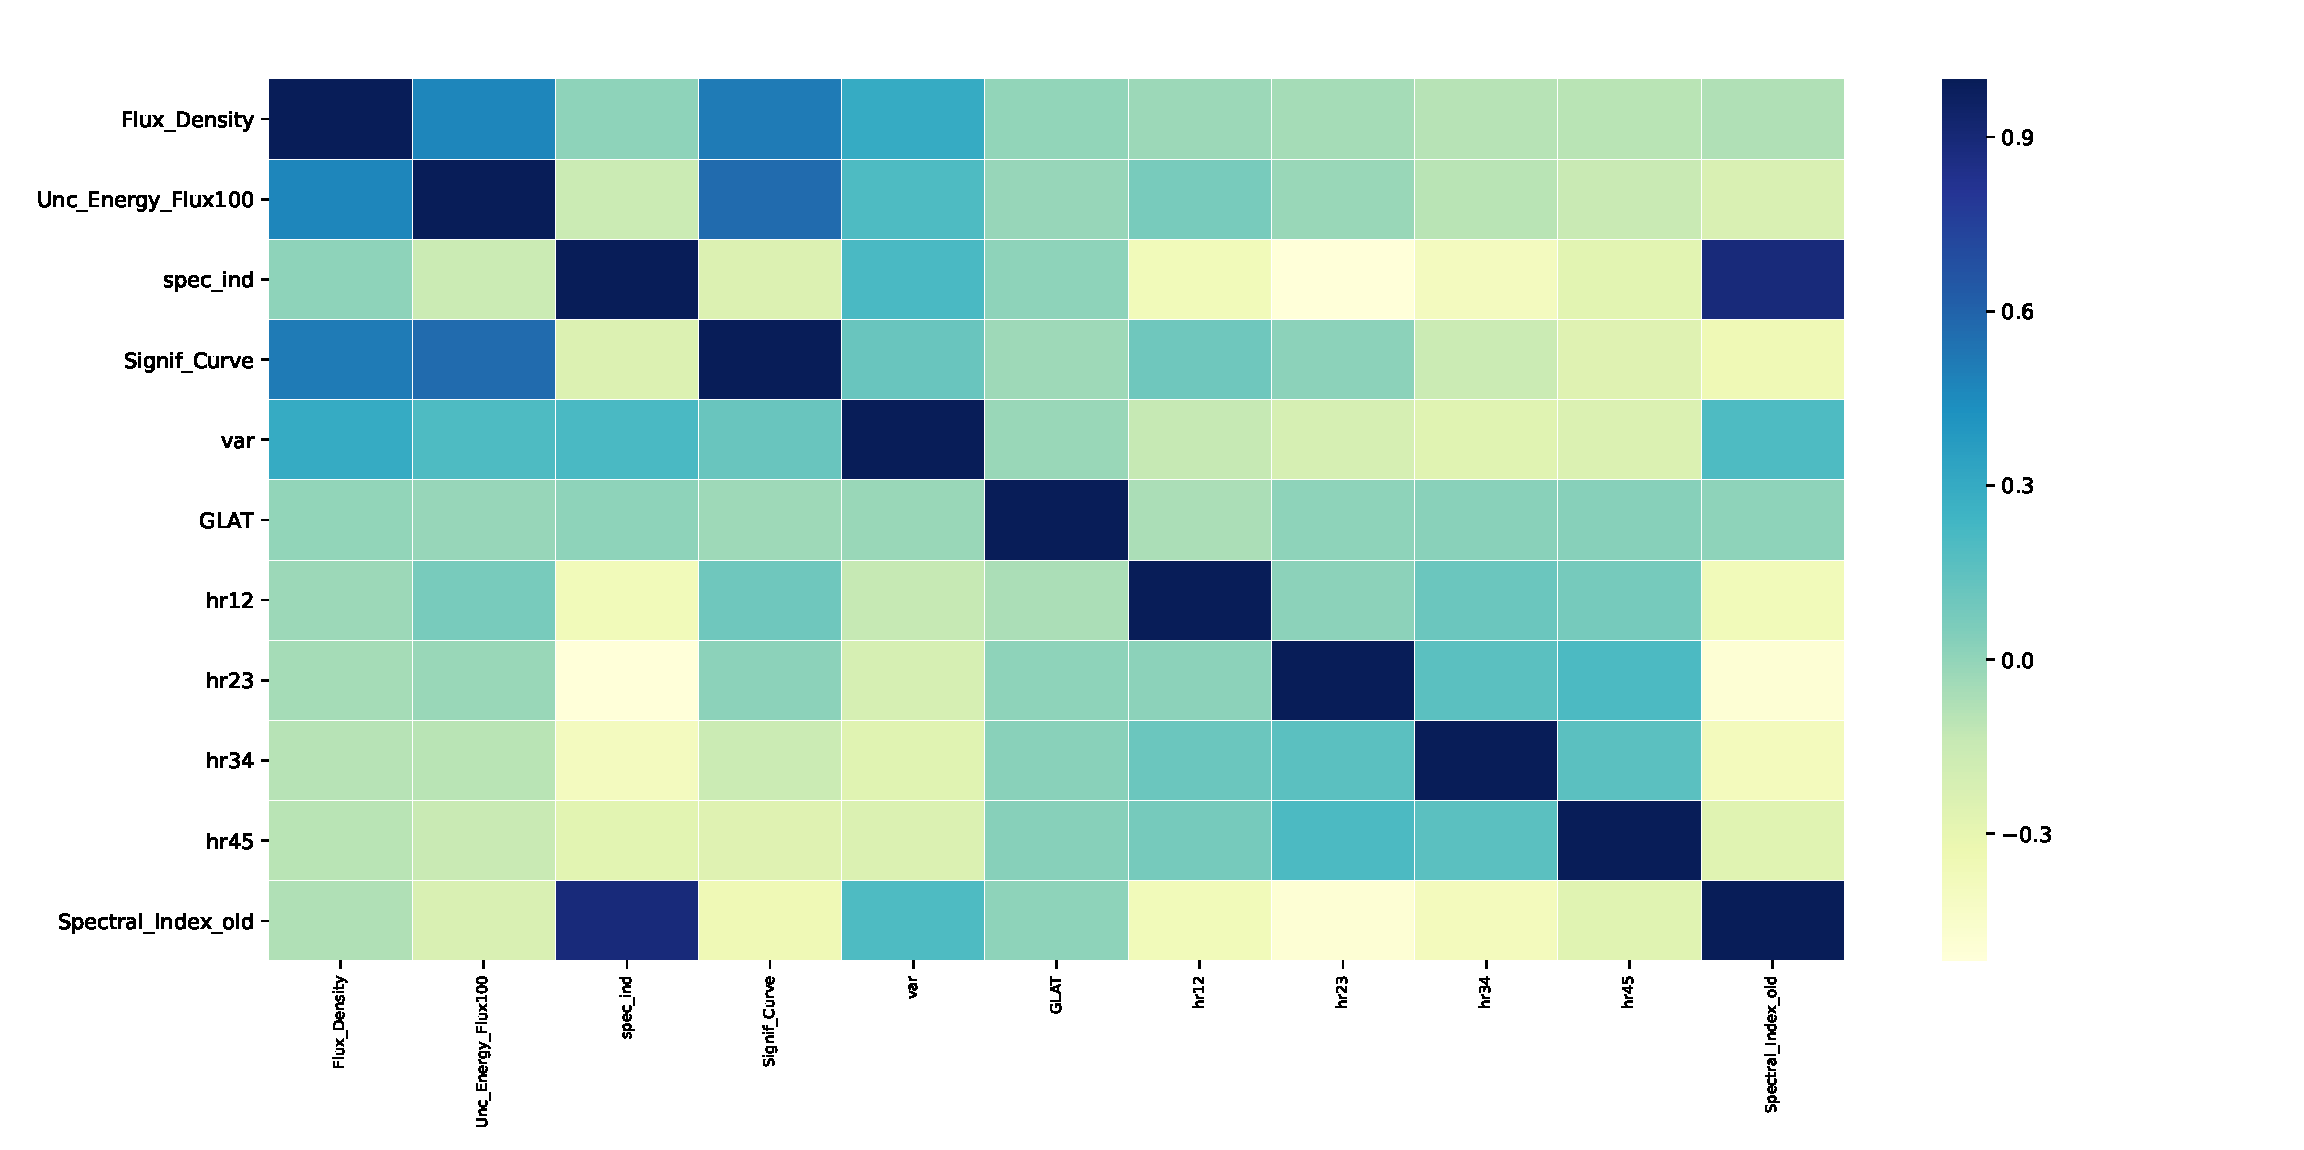
\includegraphics[width=\onepic\textwidth]{plots/correlation.pdf}
\caption{Correlation matrix for the most important features}
\label{fig:corr}
\end{figure}
[Add Table]\\

The features used for our analysis follow the same idea as the previous studies. The features, along with statistical and methodological details, are given below. A correlation matrix is presented for the most important features as well. The matrix is important for the case where there might be redundant features, in which case using only one of the two features would be a better idea.\\



[Add Table of features for both catalogs]\\

Our initial hypothesis was that certain features would be more important for classification than others. For instance, as shown below, one can see a clear distinction between the regimes of AGNs and Pulsars, based on spectral idex and significant curvature. [Add image] While not clearly obvious from the get go, we were also interested in comparing the importance of features based on the algorithms that we were using. Due to the difference in the basic method of Random Forests and Neural Networks, we expected a slight shift in their reliance on certain features. Despite that we hypothesized that features with the most contribution would be among spectral index, variability, and the curvature; as already observed by Parkinson et. al.\\

\begin{figure}[h]
%\centering
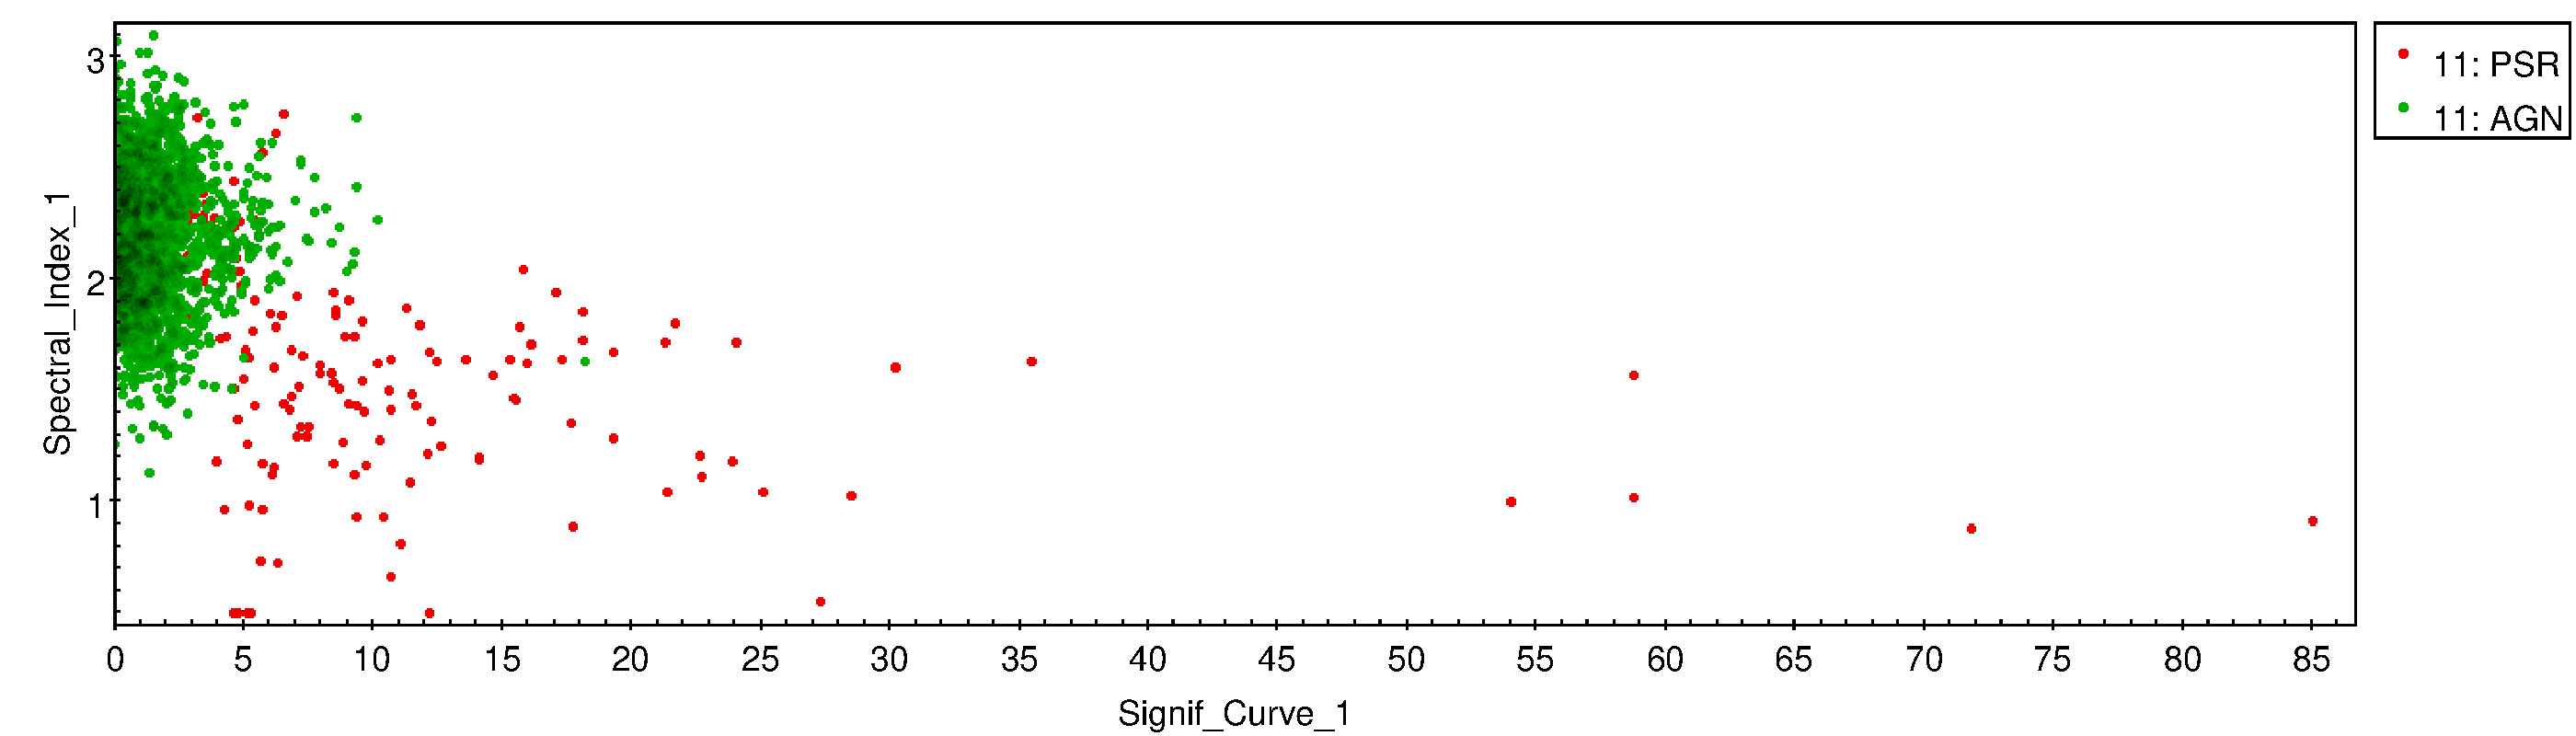
\includegraphics[width=\onepic\textwidth]{plots/signifcurvvsspecind.pdf}
\caption{Differences in AGNs and PSRs from the 3FGL catalog}
\label{fig:corr}
\end{figure}


\subsection{}


\ben
\item
Describe the features that we use for the analysis.
\item
Describe the objective function for minimization (accuracy of classification on learning sample).
Weighted objective function: give more weight to pulsars, since there are fewer of them in the catalog.
\item
Learning curve using all features?
{\it Plot: classification accuracy using the total list of features for learning and test sample as a function of complexity parameter.}
\item
Selection of the most important features.
{\it Table: features vs algorithms. Columns: algorithms, rows: features, values: significance.}
\item
Selection of meta-parameters.
{\it Plot: classification results for the test sample using a subset of features.}
\item
Train the final classifier.
{\it Table: classification accuracy of the final classifiers for different algorithms using the test sample from 3FGL.}
\een

Discuss the general features of the optimal algorithms: which features turn out to be important, what is the depth of the trees, the number of trees in random forests, the depth and number of internal nodes in the neural networks. \\

\begin{figure}[h]
%\centering
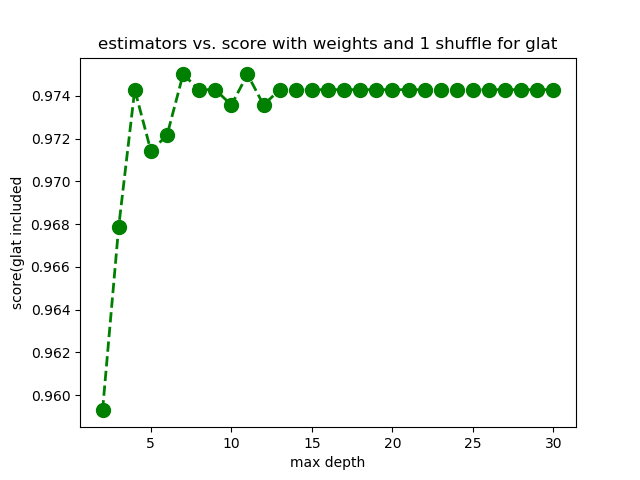
\includegraphics[width=\onepic\textwidth]{plots/Rf_maxdepth_oobscore_glat}
\caption{
Example of a figure for one column.
}
\label{fig:Maps_data}
\end{figure}


\begin{figure*}[h]
%\centering
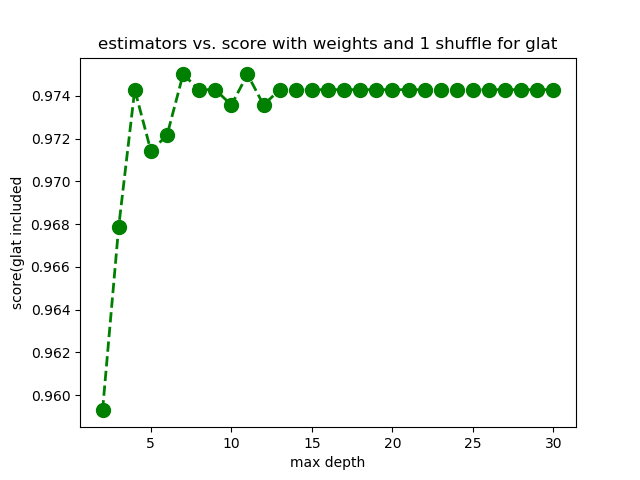
\includegraphics[width=\twopicsp\textwidth]{plots/Rf_maxdepth_oobscore_glat}
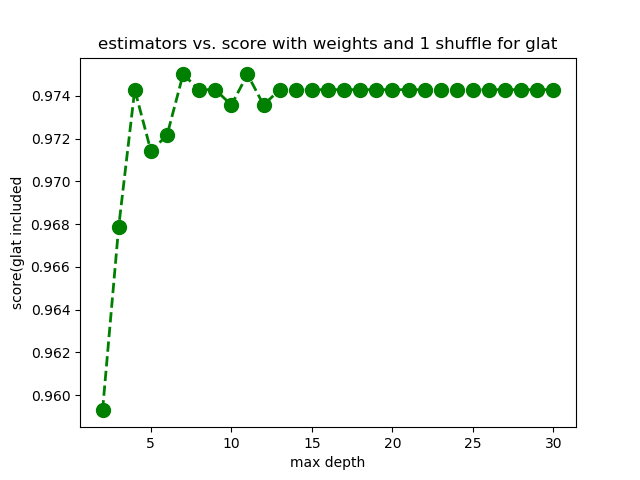
\includegraphics[width=\twopicsp\textwidth]{plots/Rf_maxdepth_oobscore_glat}
\caption{
Example of a figure for both columns.
}
\label{fig:Maps_data}
\end{figure*}

Our hypothesis about feature importances turned out to be correct, as curvature, variability, and spectral index were the most important features. The last hardness ratio was also seen to be quite important, most probably reflecting the end of the spectrum where the AGNs and PSRs shift from each other. These values are given in the table below. \\

\begin{table}[!h]
    \tiny
    \centering
    \renewcommand{\tabcolsep}{1mm}
\renewcommand{\arraystretch}{1}

    \begin{tabular}{|c|c|c|}
    \hline
    Feature Name&  RF (50,15)& GB (50,15)\\
    \hline
    Flux Density& 0 & 0        \\
    \hline
    Unc Energy Flux100& 0     & 0 \\
    \hline %\midrule   -> aakash do you mean this?
   Spectral Index & 0.16      &   0.07  \\
    \hline %\midrule   -> aakash do you mean this?
    Significant curvature& 0.28 &0.47  \\
    \hline
   var&  0.11    &  0.21  \\
    \hline %\midrule   -> aakash do you mean this?
    hr12& 0.06 &0.04 \\
    \hline
     hr23& 0.04 &0.02 \\
    \hline
    hr34& 0.06 &0.04 \\
    \hline
   hr45& 0.22 &0.10 \\
    \hline
    GLAT&0.04&0.01\\
    \hline
    \end{tabular}

    \caption{Feature importances for different Algorithm}
    \label{tab:feat_imp}
\end{table}

These importances were found to be consistent for various different algorithm parameters. So while the value might change a bit for different tree architechtures, for instance, the importances of these features were still pronounced. \\
\subsection{Comparison of the classification algorithms}

{\it Plot: classification domains for a pair of features (or different pairs of features, e.g., latitude vs index, index vs curvature, latitude vs variability).}

Probabilistic classification? Result: probability for a source to belong to a particular class.
Result of classification: table of sources with probabilities for different algorithms.
Final probability: the probability for one of the algorithms (for the most precise one?) and uncertainties determined from the other algorithms.

Discuss a few examples where algorithms give different predictions (are these sources at the boundaries of the domains).

Discuss examples where algorithms misclassify sources from the test sample.\\


In the case of test data, we worked with three different classification algortithms, namely Random Forests, Ada Boost, and Neural Networks. Here we were mostly concerned with tweaking the parameters of the classification algorithms involved, minimizing the cost of computation and aiming for the most efficient way of classification. \\

\subsubsection{Random Forests}


\begin{figure}[h]
%\centering
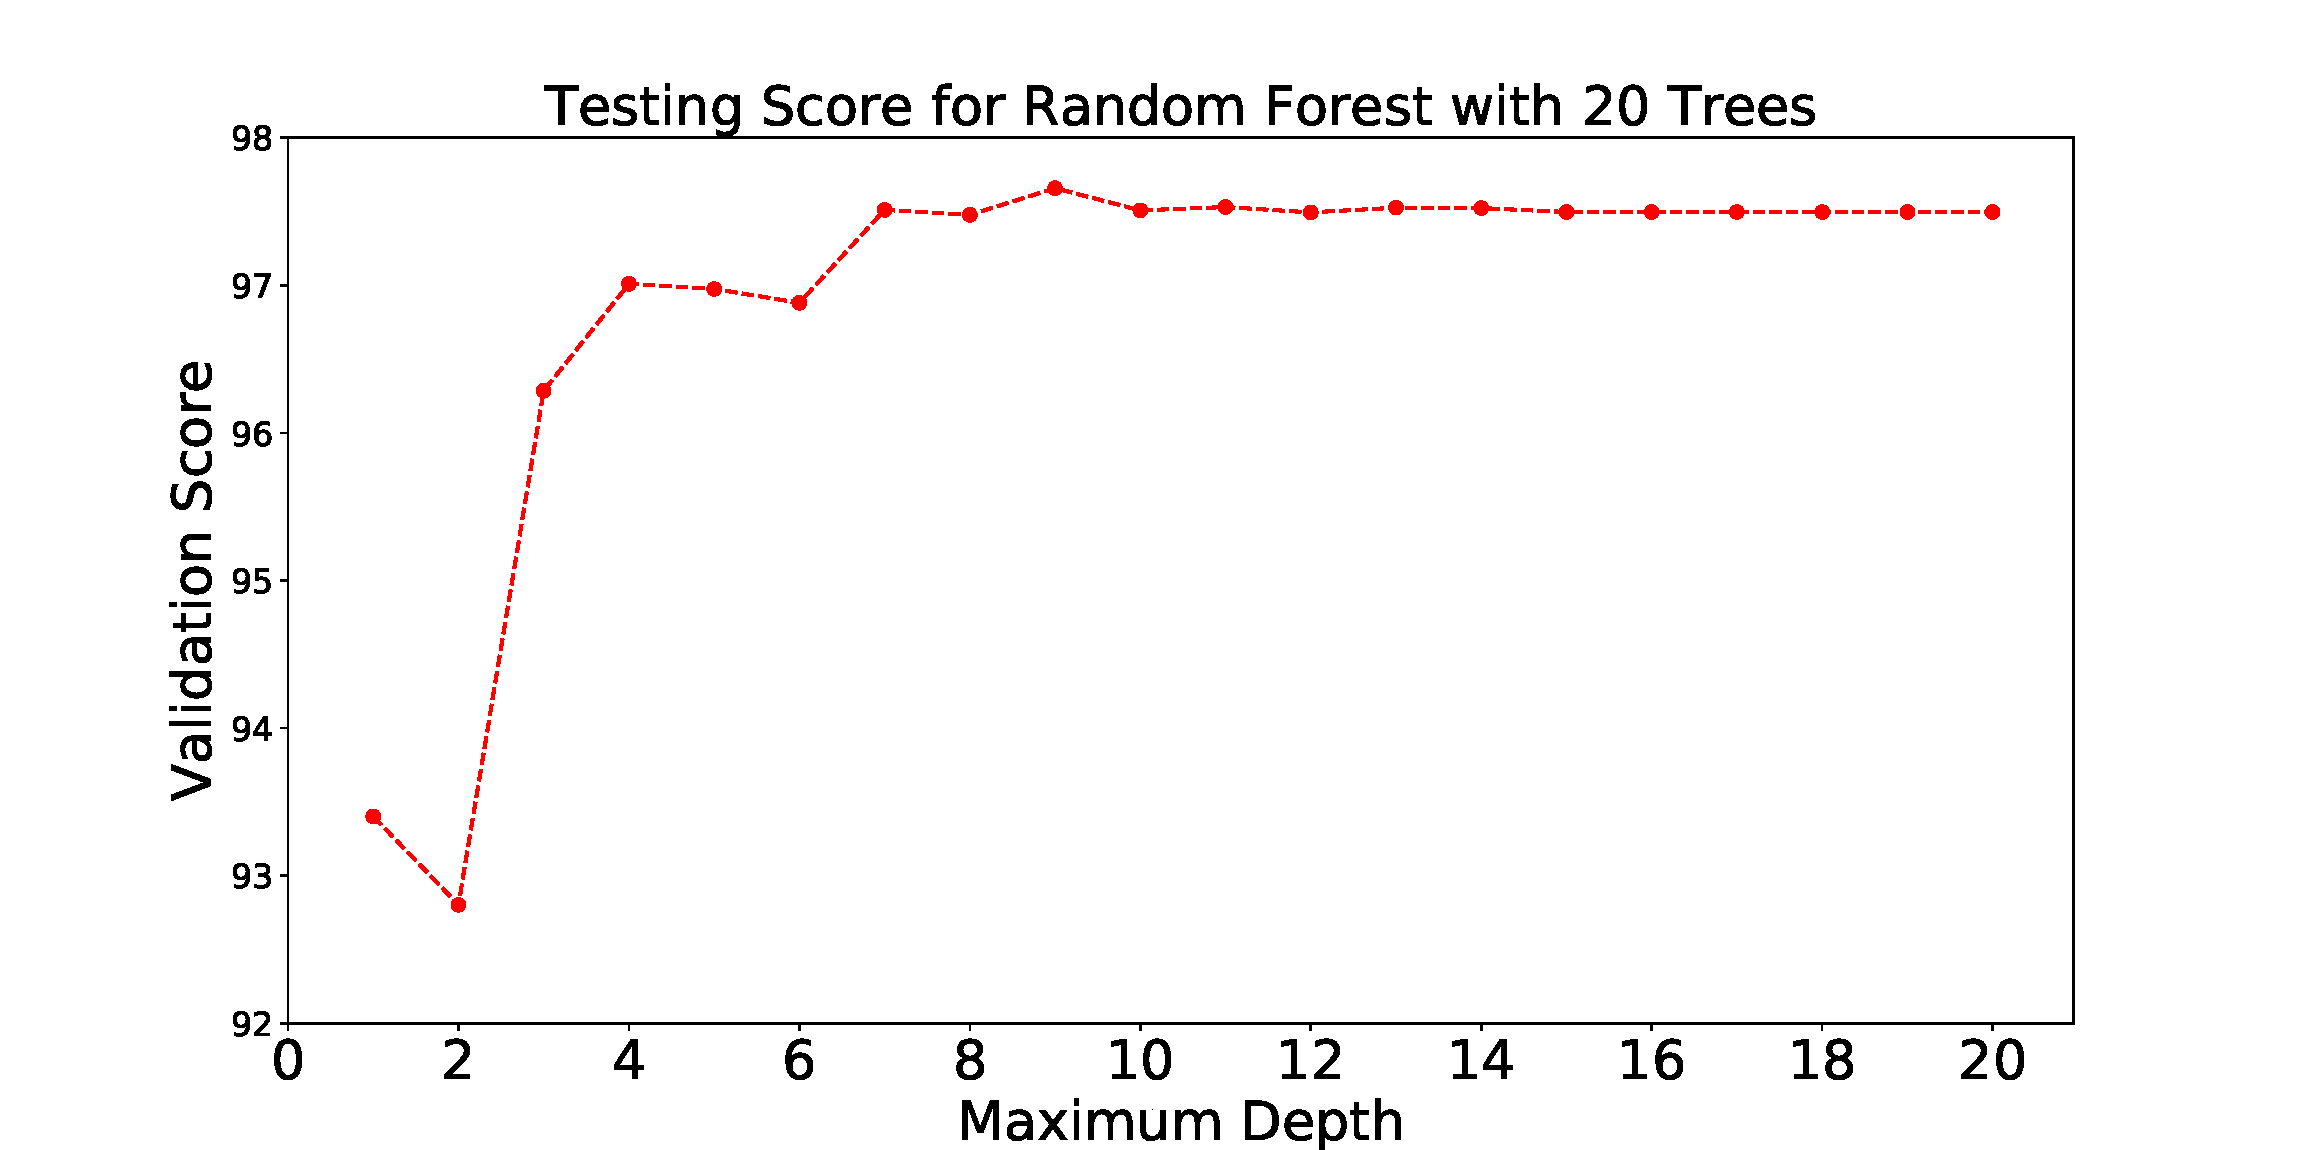
\includegraphics[width=\twopicsp\textwidth]{plots/depthvsscore_rf_10seeds_20trees.pdf} \\
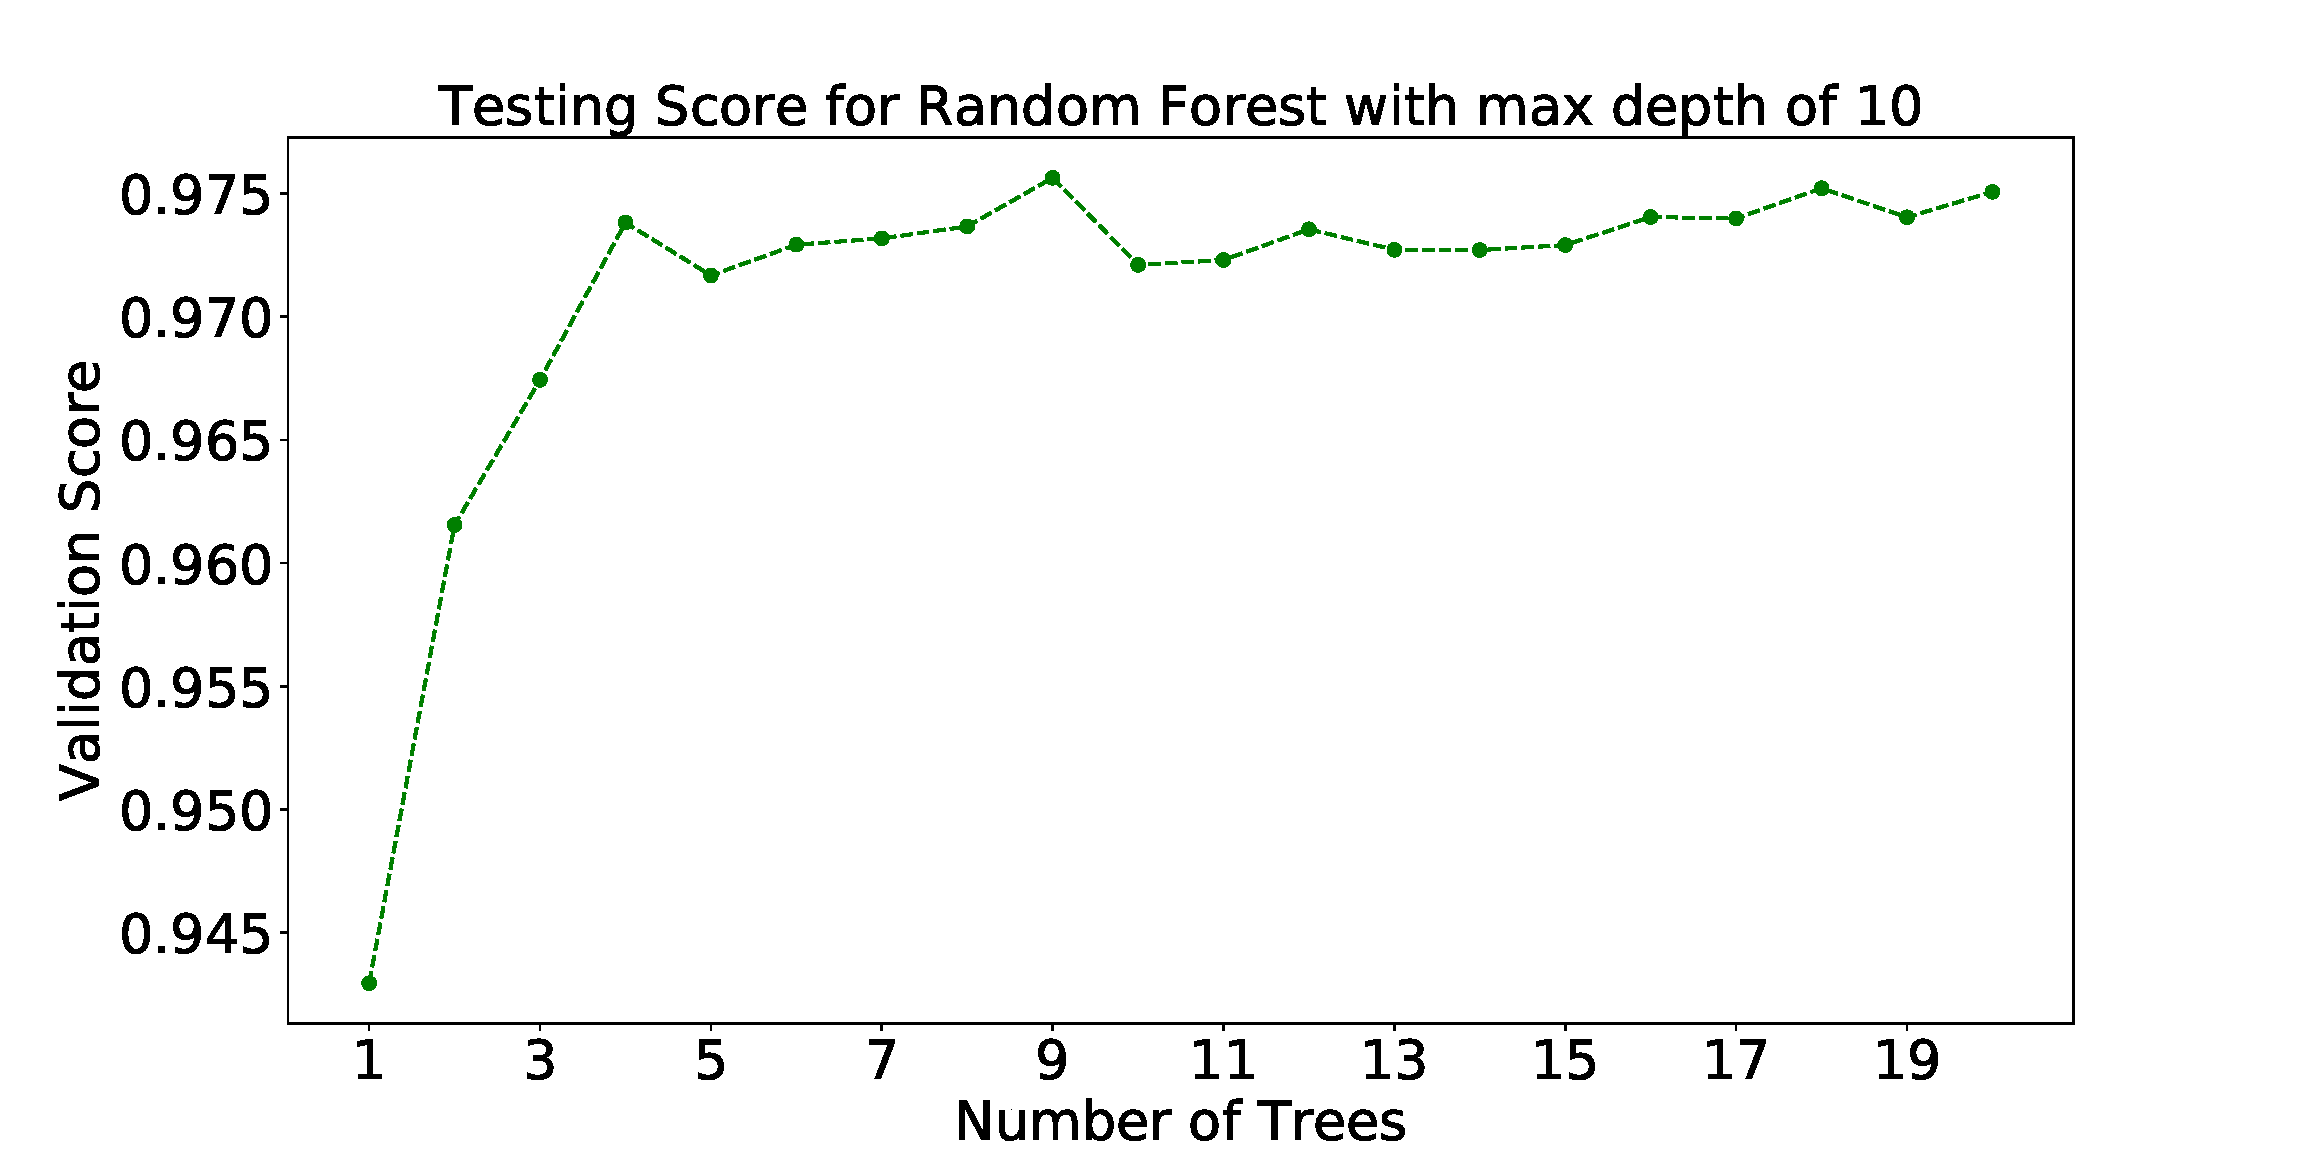
\includegraphics[width=\twopicsp\textwidth]{plots/treesvsscore_RF_10seeds_10maxdepth}
\caption{
Random Forests on Testing Data
}
\label{fig:Maps_data}
\end{figure}

The two main parameters involved in Random Forests are the number of trees and the maximum depth of the trees involved. Figures below shows one instance of the accuracy as a function of maximum depth when the number of trees was kept constant, and as a function of number of trees when the maximum depth was kept constant. \\


\subsubsection{Neural Networks}

In the case of neural networks we were concerned with the number of epochs that one would need to tweak, along with a dependence on the number of neurons in the hidden layers. A final improvement involved checking whether multiple hidden layers would actually add to such a classification algorithm or not.\\
As can be seen in the figure, a complex network with two hidden layers (100 and 5 neurons) reaches the maximum accuracy pretty fast. The results becoming more consistent at higher epochs. A similar result was found for a network having two hidden layers but with only 20 neurons in the first layer. However, such networks could also lead to overtraining, and therefore it is important to check whether such a high accuracy could perhaps be reached by less complicated algorithms, which would drastically reduce the chances of overtraining and allow for a more flexible classificaition methodology.\\

\begin{figure}[h]
%\centering
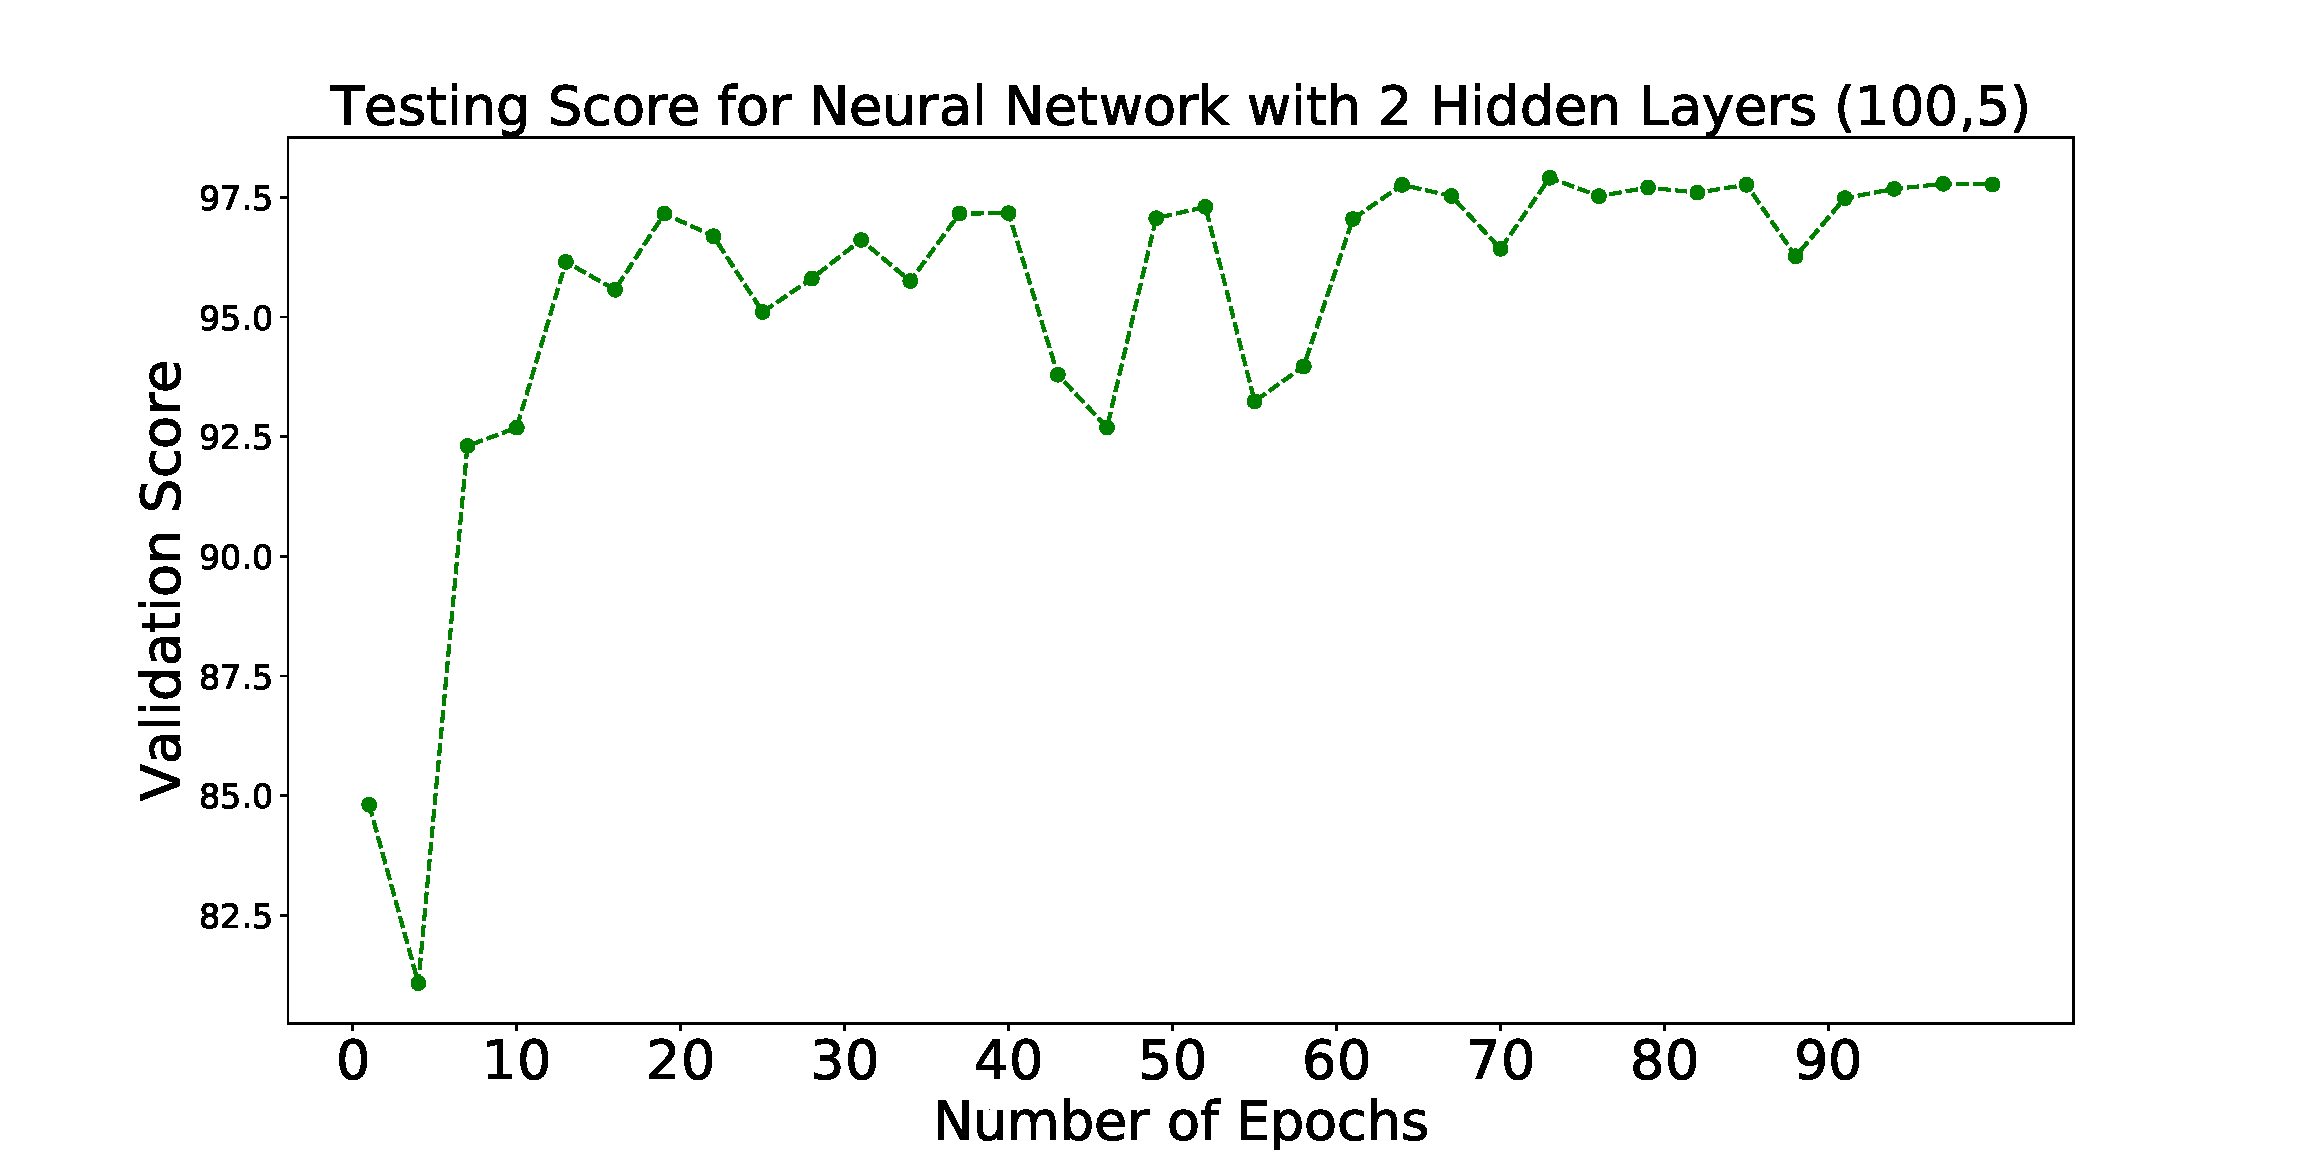
\includegraphics[width=\onepic\textwidth]{plots/epochsvsscore_10seeds_100_2}
\caption{
Example of a figure for one column.
}
\label{fig:Maps_data}
\end{figure}

\begin{figure}[h]
%\centering
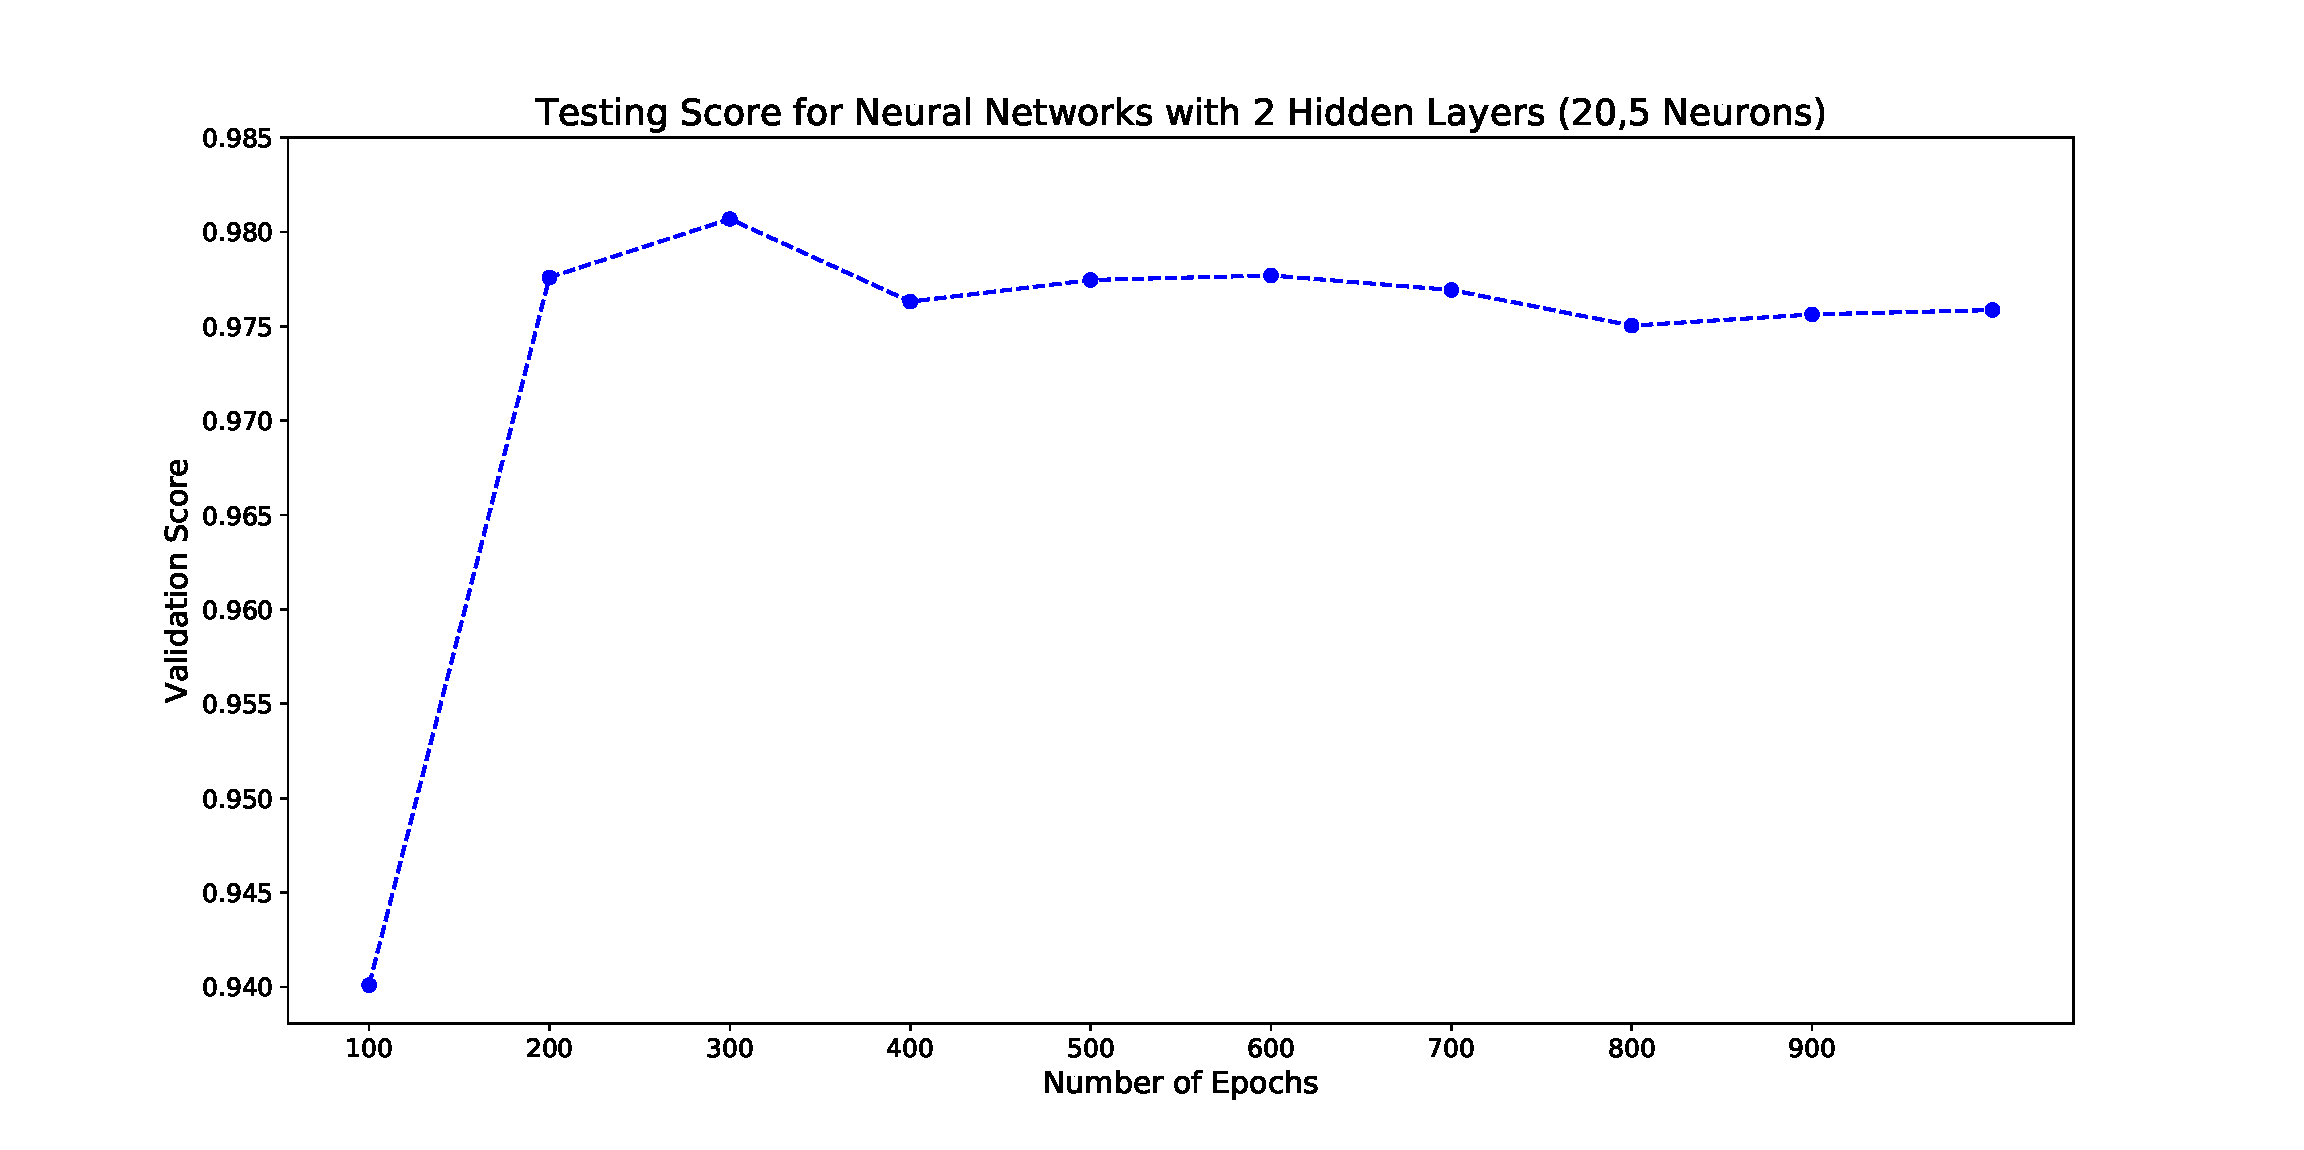
\includegraphics[width=\onepic\textwidth]{plots/epochsvsscore3_10seeds.pdf}
\caption{
Neural Network
}
\label{fig:Maps_data}
\end{figure}

A consistent and accurate result is found even for networks with only one hidden layer with 20 and 5 neurons in the hidden layer respectively. There seems to be no significant dependence for the number of epochs above 30, and even a simple network with one layer and 5 neurons shows a high accuracy for only 30-40 epochs.\\


\begin{figure*}[h]
%\centerin
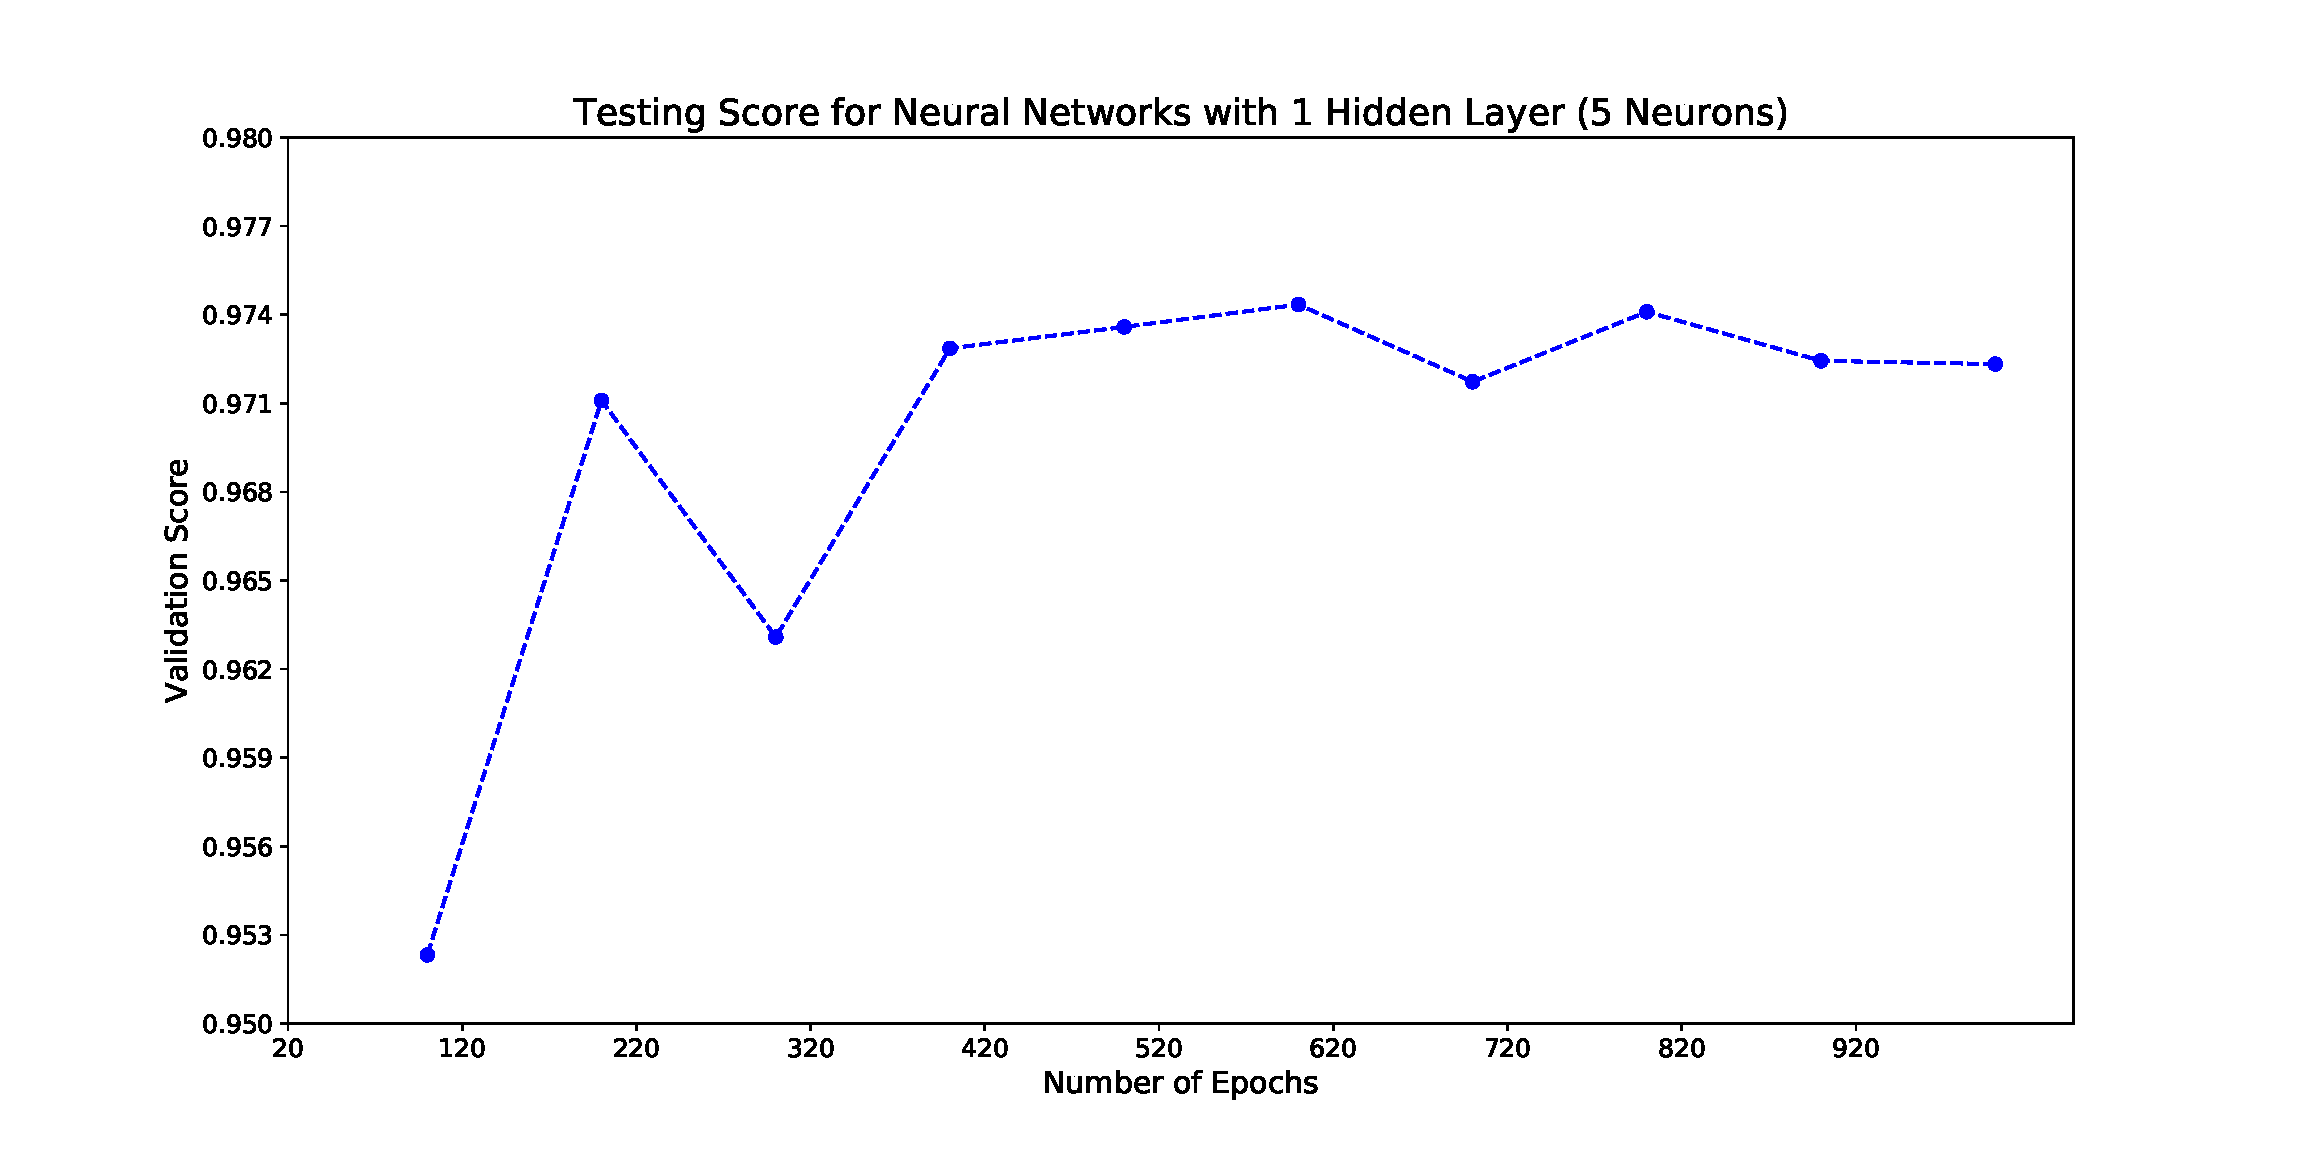
\includegraphics[width=\twopicsp\textwidth]{plots/epochsvsscore1_10seeds.pdf}
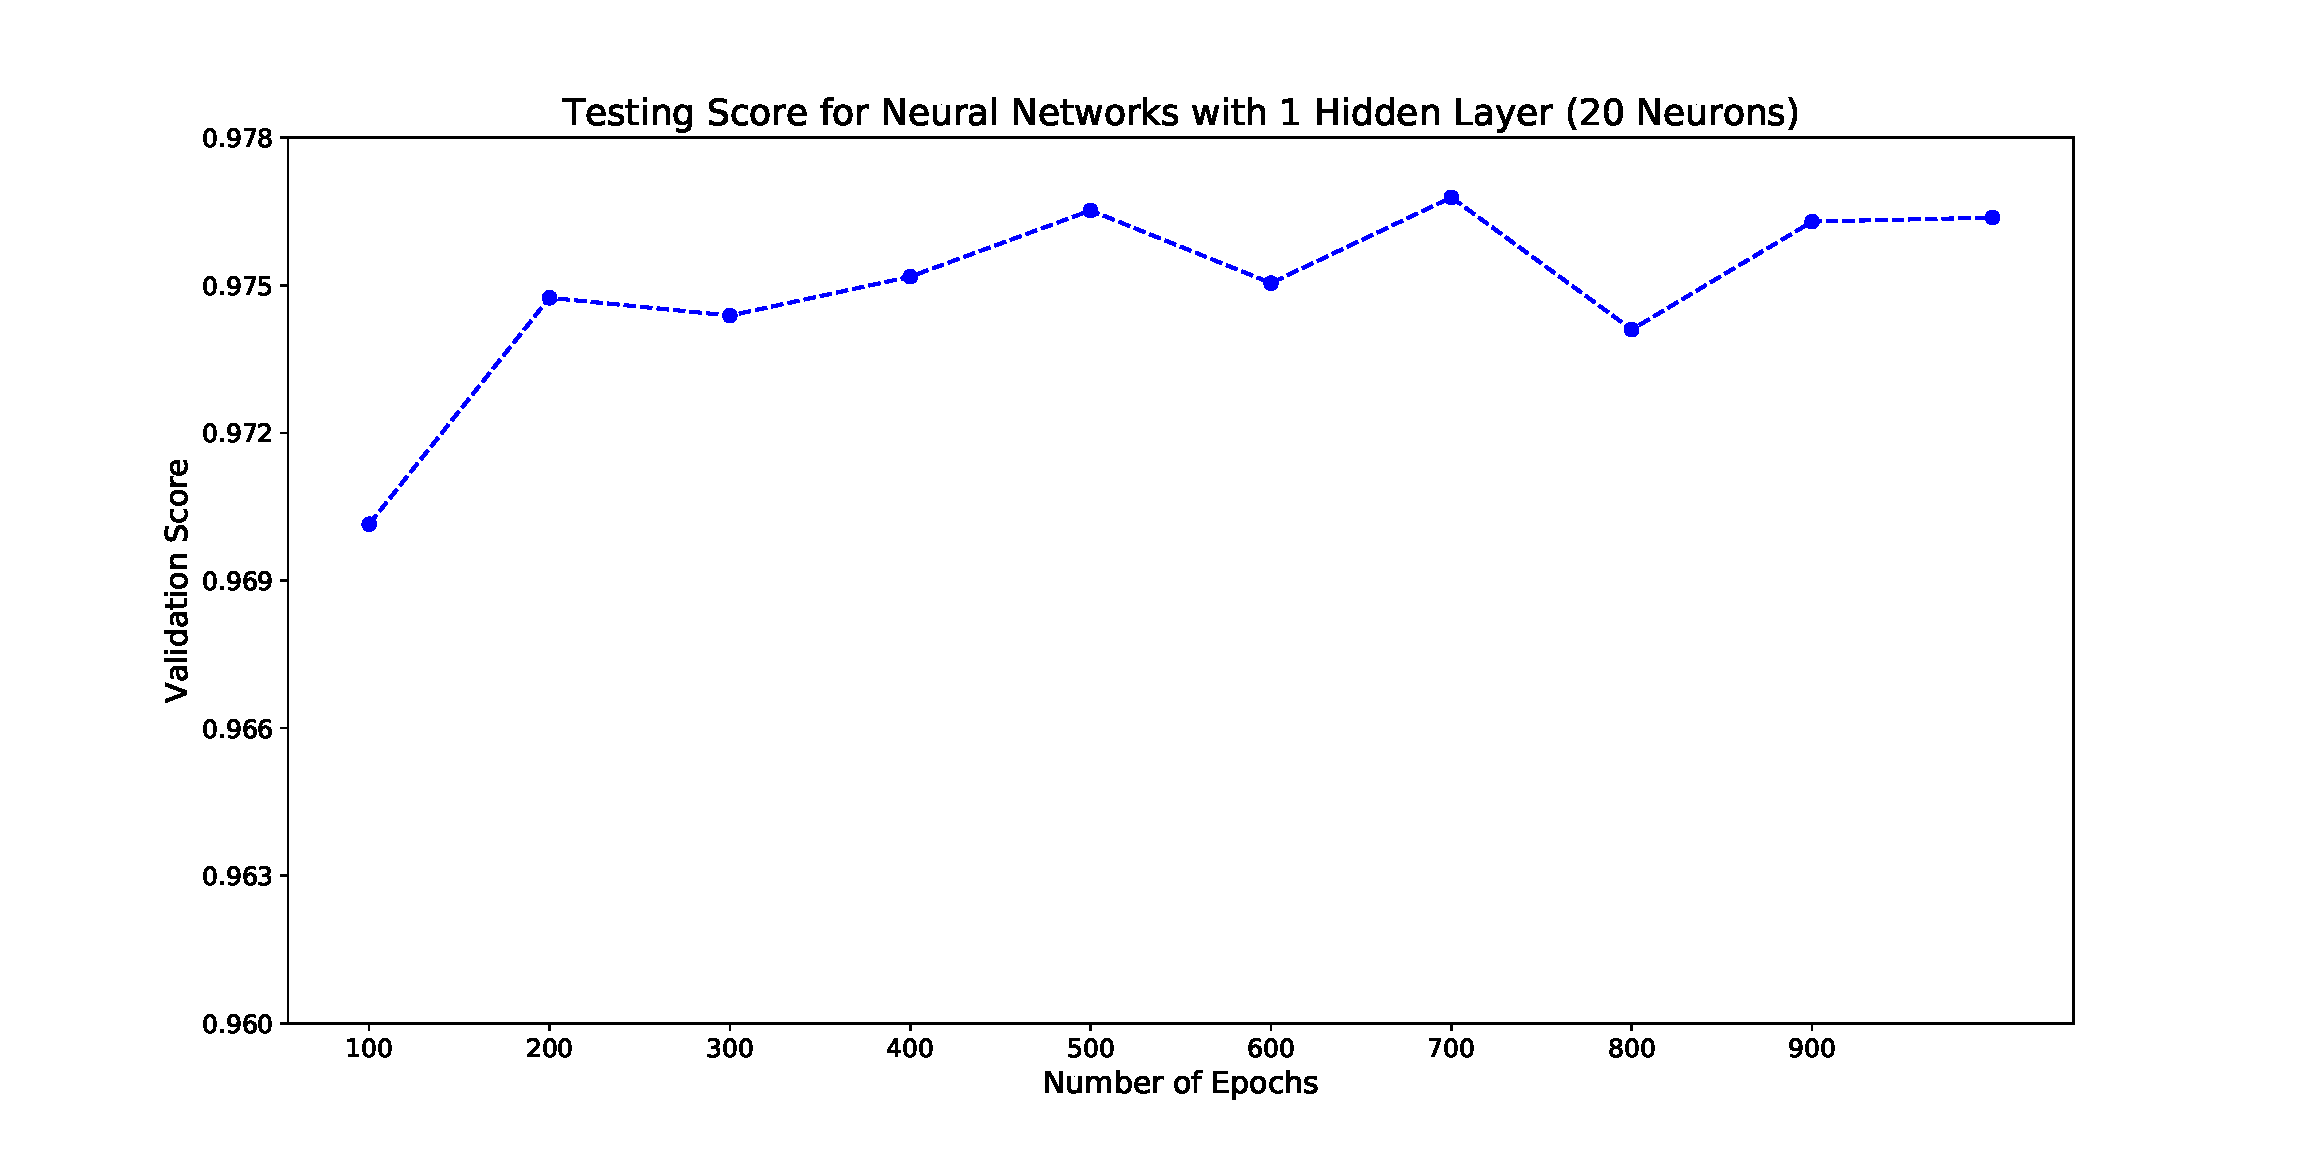
\includegraphics[width=\twopicsp\textwidth]{plots/epochsvsscore2_10seeds.pdf}
\caption{
Neural networks
}
\label{fig:Maps_data}
\end{figure*}

\begin{figure}[h]
%\centering
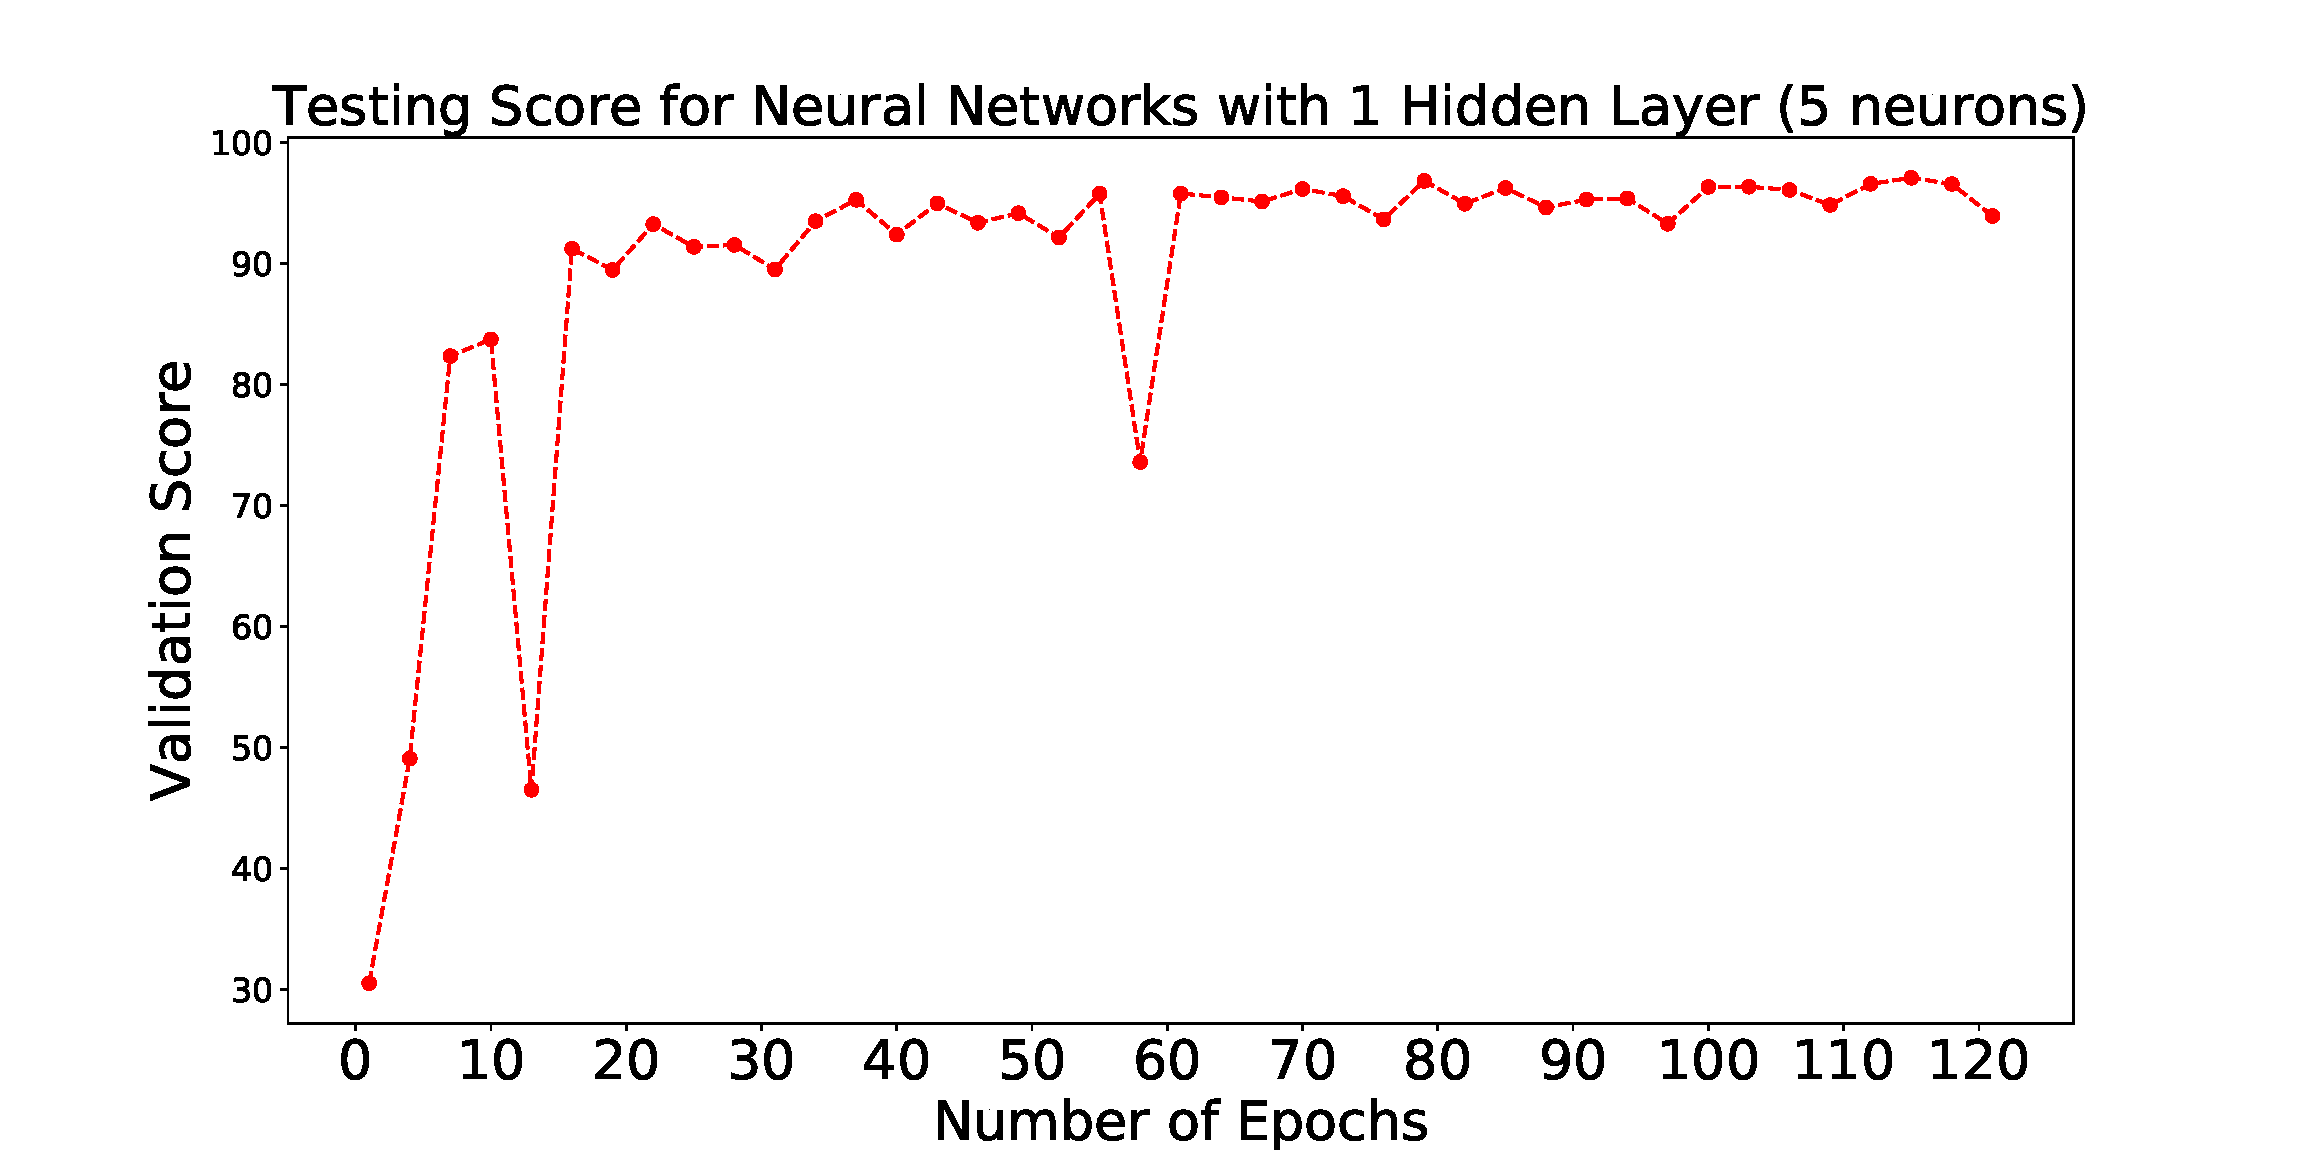
\includegraphics[width=\onepic\textwidth]{plots/epochsvsscore1_10seeds_1layer_5.pdf}
\caption{
Neural Network
}
\label{fig:Maps_data}
\end{figure}	



